\section{Product perspective}
The aim is to build a system that manage the users’reservations and grants the possibility of booking the place in queue without wasting time while they're waiting their own turn outside the market. 
\par
--The system have to provide User infomation about queue's dynamic in real time (i.e the number of people ahead and the time estimation before his own turn). --
To do this, the application should try, in the best way, to estimate the time that the customers will spend in the shop, in order to notify in time users who are waiting their turn. 
\\
The application analyses the customers’ statistics and computes the average shopping time.
The calculation considers the time range between the moments in which the User goes in and out.  
\par
In this way, the customers in queue will be notified in time and will be able to use GoogleMaps APIs to compute the path for arriving in time to market. 
The choice of using Google Maps APIs derives from the easy usability, frequency update and very large documentation.
\par
Moreover, it will be possible to book a visit choosing the date and time in advance (of some days?). In this case, users will also have to indicate an approximation of the shopping time. 
\\
The time will be splitted into 30 minutes slots, and customers will choose which they want among the free ones. \par
\bigskip
In the UML diagram below will be list the main classes in order to understand how the whole system works.
\par 
\bigskip
\bigskip


\begin{figure}[h]
  \caption{Class diagram with UML}
  \label{fig:UML}
  \centering
  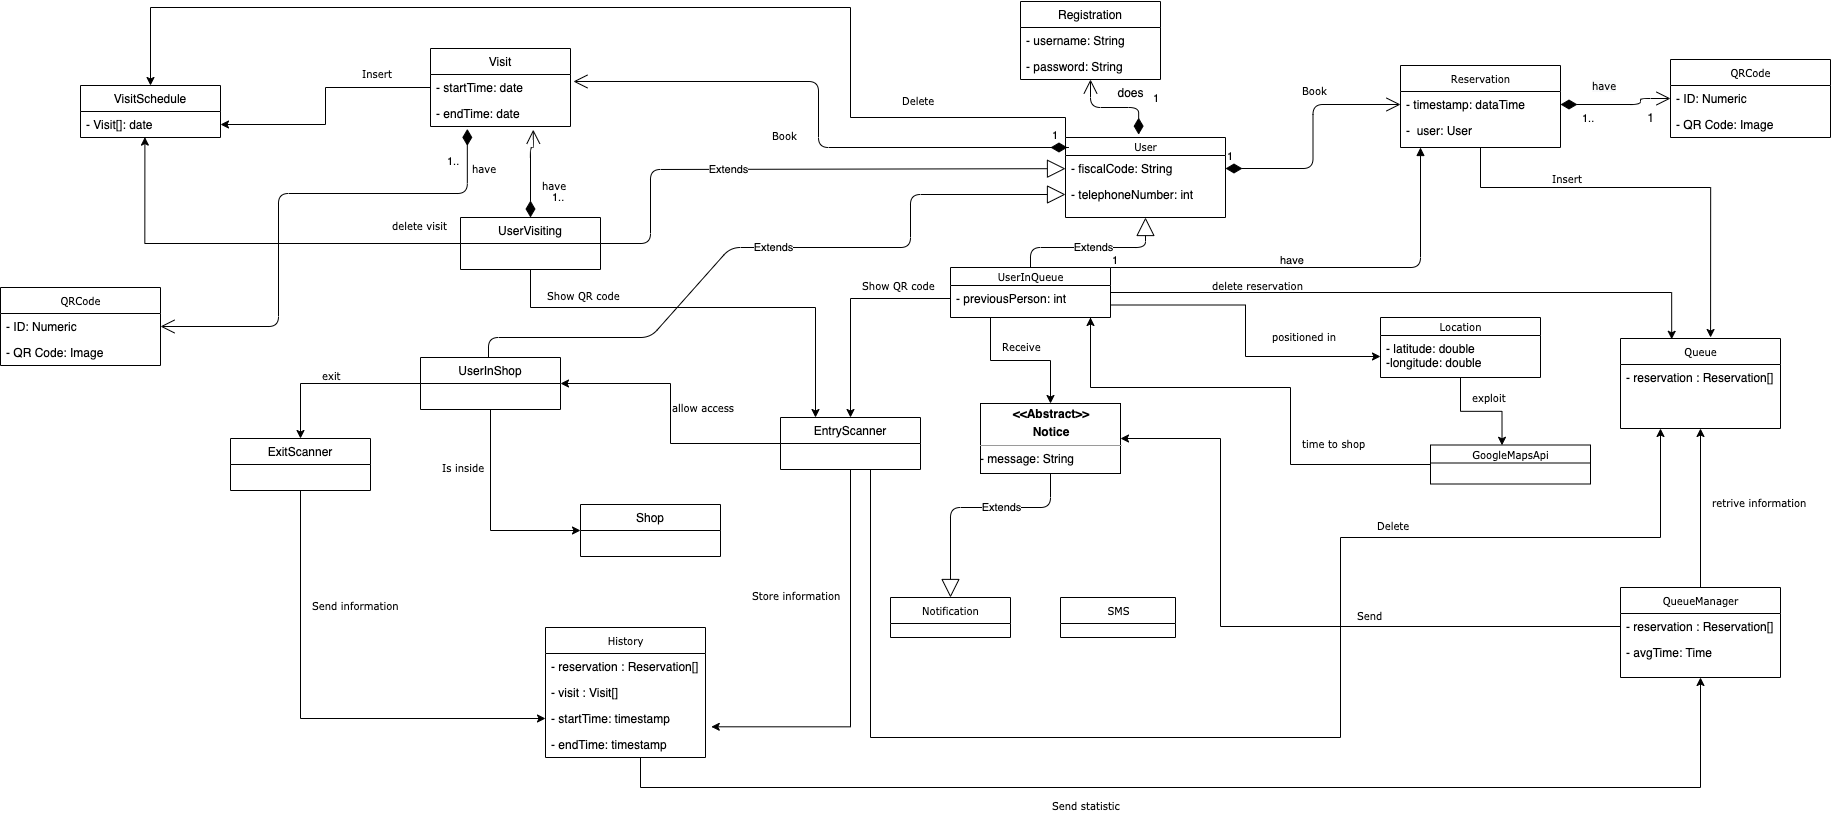
\includegraphics[width=1\textwidth, height=0.6\textwidth]{diagrams/2-UML.png}

\end{figure}
\par 
\medskip
As we can see from the class diagram in figure ~\ref{fig:UML}, the user can book once or a visit or a reservation.
In both cases will be provide him a QRcode, which will be submit to enter in the market. 
If the the User decided to undo his reservation in the queue could do it by making a cancellation from the application. 
\par
\medskip
Moreover, if the User allows to share his position, the system will notice him in advance due to his punctuality.
\\
In addition the system will notice the User through an SMS or a notice when it's almost his turn (10-15 minutes before).
\\
Now we will analyze the interaction between the User and the system, in order to understand possible criticities.
\par 
\bigskip

\begin{figure}[h]
  \caption{State diagram of the reservation in the queue}
  \label{fig:Reservation}
  \centering
  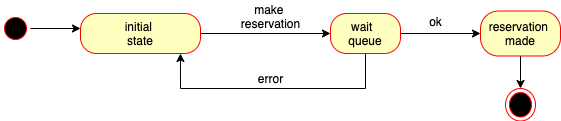
\includegraphics[width=1.1\textwidth, height=0.3\textwidth]{diagrams/2-reservation.png}

\end{figure}
\par 
\medskip

In the Figure ~\ref{fig:Reservation} first state diagram it can be osserved how a generic User can make a reservation thorugh the system. It's sufficient making this action to be added in queue to enter in the market.
\\If something goes wrong the User will be redirect to the home screen (initial state).
\\Usually the system reject the request if the market is next to closure (or for logistic problem).

\par 
\medskip

\begin{figure}[h]
  \caption{State diagram of booking a visit}
  \label{fig:Visit}
  \centering
  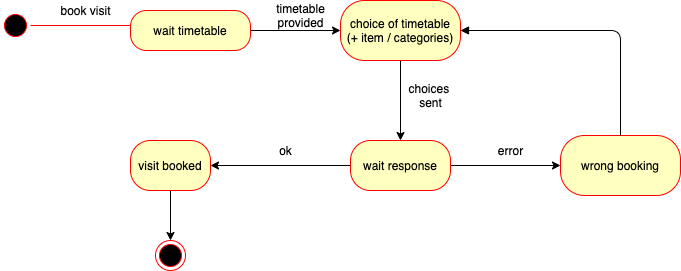
\includegraphics[width=0.8\textwidth, height=0.4\textwidth]{diagrams/2-visit.png}
\end{figure}

\par 
\medskip

The Figure ~\ref{fig:Visit} explains instead how to book a visit in the market. Once the timetable is provided, the User have to select the range time of the visit and the items that he wants to purchase. \par If the choice made by the user is wrong (i.e timetable's slot full), the system notify him; the User will try again until his choice is correct.
\par 
\medskip


\section{Product functions}
\subsection{Queue Manager}
The most important function is the \textit{Queue Manager} because it must avoid the users waiting too much time their turn due to a wrong use of notifications. [TODO]
In fact, it have to foresee, through statistics from users’ information, the correct time in which the users will enter in the market once arrived. This can be done thanks to the notifications sent to the user 
It will also have to understand when accept and when refuse reservations, according to shop closing time and the number of people in queue. 
\subsection{Data Collection}
The \textit{Data Collection} is essential for the correct behavior of the Queue Manager described previously, because it will have to provide precise dates according to client’s information. 
Therefore, the system will have to ask clients precise questions according to keep useful informations for estimating the shopping time into the supermarket, without violating users’ privacy. 
\\
In order to achieve this goal, it needs to oblige the user to register himself in the system and to check the item to allow the processing of his personal data, necessary to reserve virtually the seat in the queue.
\\
One of the possible information asked could be the dimension of the expenses, which can be estimate by the number of item that are going to be purchased. This will be used, with the entry time, to track the number of user inside the market who is finishing. Then will be possibile to notify in advance users in queue about the closeness of their turn.

\section{User characteristics}
We distinguish the actors into our application based on actions and interactions with the external world:

\begin{itemize}
\item \textit{User}: he’s a client who has signed in the system and he can book a visit or take his queue number.
\item \textit{UserInQueue}: he’s a User who has taken his own turn in queue and he’s waiting for the system notification
\item \textit{UserVisiting}: he’s a User who has booked a visit and he’s still waiting for entering into the supermarket.
\item \textit{UserInShop}: he’s a client who has taken his own queue ticket or he has booked a visit. After that he is arrived at the supermarket, he has scanned the QR code and he has entered into the shop.
\end{itemize}


\section{Assumptions, dependencies and constraints}
